\section*{Problem 4: Project Milestone}

Build a simple object dection model. Our object detector will comprise of a
binary classifier per category: given features of an image patch corresponding
to a bounding box, does this patch contain an object of the category of
interest?

\subsection*{Solution}

\subsubsection*{Experimental Setup}

I treated this problem as a multi-label classification problem. Each image patch
may contain objects from one of 17 categories that are part of the
\texttt{vehicle} or \texttt{animal} supercategories in the
\href{http://cocodataset.org/}{COCO dataset}\footnote{I chose to use these 17
  categories instead of all 80 to simplify the problem and reduce training
  time.}.

Region proposal for patches were found with the selective search fast
algorithm\footnote{Jasper RR Uijlings, Koen EA van de Sande, Theo Gevers, and
  Arnold WM Smeulders. Selective search for object recognition. International
  journal of computer vision, 104(2):154-171, 2013.} Then, the bounding box
coordinates were projected and turned into features with adaptive max pooling.

Negatives could then just be patches that don't contain a specific
category. Additional patches that contain objects of no categories could be
added, but I didn't find this helpful. Mining hard negatives didn't seem to do
much either.

After training, validation, and test datasets were created, various models were
tried. The best model was that with the lowest cross-entropy loss on the
validation dataset. Models tried were logistic regression, a multi-layer
perceptron with 1 layer of hidden units, and a multi-layer perceptron with 2
layers of hidden units. $L_2$ regularization was applied in all the models.

\subsubsection*{Model Selection}

The best model was the multi-layer perceptron with 2 layers of hidden units. The
first layer had 512 units, and the second layer had 256 units. The loss and
average precision score on the training and validation dataset can be seen in
Figures \ref{fig:4loss} and \ref{fig:4average_precision_score}. The best metrics
are summarized in Table \ref{tab:4training_summary}.

\begin{figure}
  \centering
  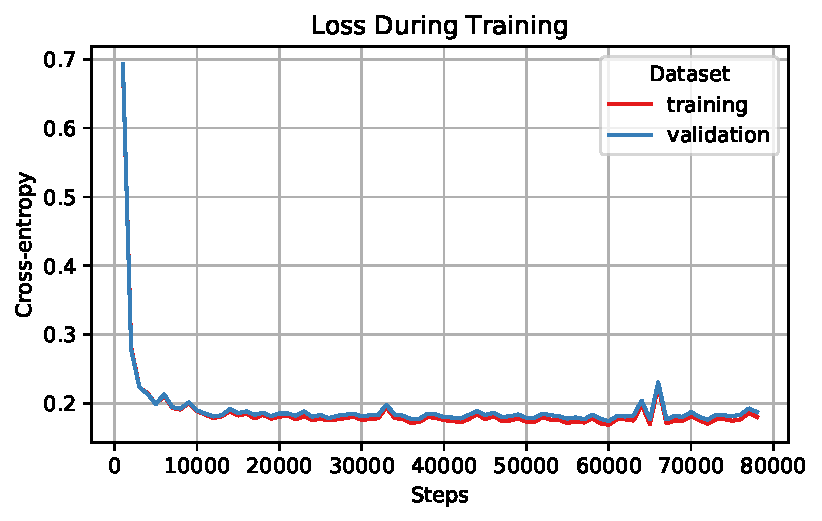
\includegraphics{problem4/loss.pdf}
  \caption{The loss between the training and validation dataset is rather small,
    which indicates the choice of $\lambda$ was appropriate.}
  \label{fig:4loss}
\end{figure}

\begin{figure}
  \centering
  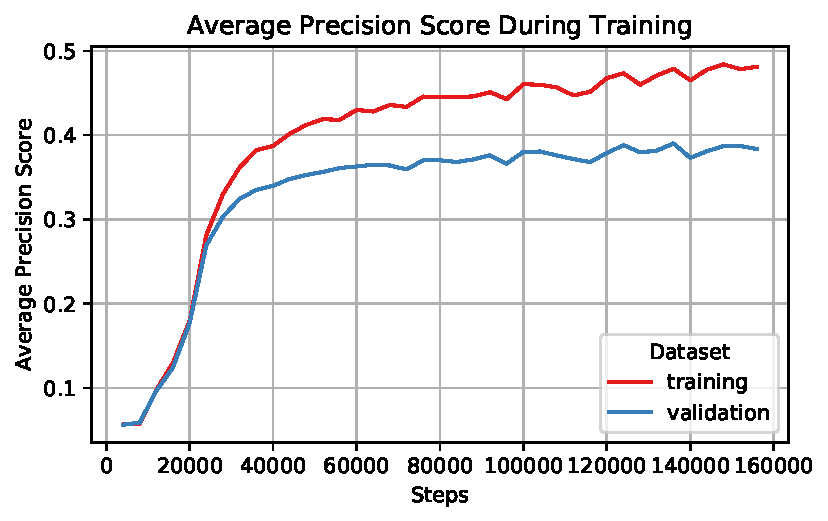
\includegraphics{problem4/average_precision_score.pdf}
  \caption{The average precision score is averaged over the categories without
    weighting.}
  \label{fig:4average_precision_score}
\end{figure}

\begin{table}
  \centering
  \begin{tabular}{lrr}
\toprule
{} &  Average Precision Score &      Loss \\
\midrule
Training   &                 0.483937 &  0.136209 \\
Validation &                 0.390272 &  0.148008 \\
\bottomrule
\end{tabular}

  \caption{The best loss and average precision score achieved during training.}
  \label{tab:4training_summary}
\end{table}

For the $L_2$ regularization parameter, $\lambda = 0.004$ was found to work
best. A smaller parameter led to overfitting as seen by a big gap between loss
on the training dataset and validation dataset. A larger parameter led to a
degredation in performance on the validation dataset.

For the optimization, stochastic gradient descent was used with Nesterov's
momentum. The learning rate was $0.05$, and momentum was $0.9$. The batch size
was 16.

\subsubsection*{Evaluation}

The best model was evaluated against the test dataset. On the test dataset, the
average precision score was
$0.254112$. The numbers are broken out
by category in Table \ref{tab:4average_precision_score_by_class}.

\begin{table}
  \centering
  \begin{tabular}{lrrr}
\toprule
      Label &  Training Observations &  Test Observations &  Average Precision Score \\
\midrule
    bicycle &                   2166 &                416 &                 0.130984 \\
        car &                  12179 &               2476 &                 0.463947 \\
 motorcycle &                   2630 &                614 &                 0.310926 \\
   airplane &                   3045 &                447 &                 0.465379 \\
        bus &                   2972 &                543 &                 0.306217 \\
      train &                    873 &                160 &                 0.245715 \\
      truck &                   6058 &               1238 &                 0.221581 \\
       boat &                   2961 &                650 &                 0.265335 \\
       bird &                   6485 &               1473 &                 0.368913 \\
        cat &                   2516 &                569 &                 0.516294 \\
        dog &                   3387 &                562 &                 0.268118 \\
      horse &                   4802 &               1074 &                 0.282166 \\
      sheep &                   7702 &               1378 &                 0.473883 \\
        cow &                   7733 &               1582 &                 0.351056 \\
   elephant &                   5177 &                853 &                 0.530496 \\
       bear &                    851 &                113 &                 0.130927 \\
      zebra &                   5147 &               1153 &                 0.661771 \\
    giraffe &                   3908 &                826 &                 0.738177 \\
\bottomrule
\end{tabular}

  \caption{Generally, less frequently occuring categories have lower scores.}
  \label{tab:4average_precision_score_by_class}
\end{table}

\subsubsection*{Discussion}

The linear model essentially does a logistic regression for each category. The
advantage of the multi-layer perceptron is that the weights for the non-terminal
layers are shared between each categories. Thus, if one believes that the hidden
units are learning an intermediate representation of the image, categories with
not so many examples can leverage what is learned from the more abundant
categories.

In reality, the multi-layer perceptron only gives us a $0.03$ boost in average
precision score over the linear model, so it's questionable if the additional
complexity is worthwhile.
